\Chapter{Pairings\label{hfdst-pairings}}

In dit hoofdstuk zal de werking van pairings wiskundig uit de doeken gedaan worden. Meer specifiek zal de Tate pairing bestudeerd worden. Er zal duidelijk gemaakt worden hoe de pairing berekend kan worden. Vervolgens worden enkele schema's voorgesteld die gebruikt kunnen worden voor versleuteling van gegevens en de aanmaak van digitale handtekeningen. In het volgende hoofdstuk wordt dan een schakeling ontworpen waarmee de Tate pairing berekend kan worden.

Enkel de hoogstnodige theorie zal hier behandeld worden. Voor een meer diepgaande uiteenzetting wordt als startpunt opnieuw verwezen naar \cite{maas}. Het is uit dit werk dat de informatie in de volgende paragrafen afkomstig is, tenzij anders vermeld.

\section{Inleidende wiskunde}

Alvorens de wiskundige theorie van pairings nader bekeken wordt, dient die van elliptische krommen duidelijk gemaakt te worden. Het is met behulp van deze constructies dat pairings berekend kunnen worden. Elliptische krommen worden doorgaans gedefinieerd over een eindig veld. Vandaar dat de noodzakelijk theorie van beiden hier even heel kort herhaald wordt.

\subsection{Eindige velden}

Een eindig veld $\mathbb{F}_q$ wordt gedefinieerd door zijn karakteristiek $q$. Die karakteristiek is bij cryptografische toepassingen doorgaans een groot priemgetal $p$ of 2, hoewel tegenwoordig ook onderzoek gedaan wordt naar toepassingen met een karakteristiek 3. Een veld zonder zijn nul element wordt aangeduid als
\[\mathbb{F}_q^* = \mathbb{F}_q \setminus \{ 0 \}.\]

Volgens de kleine stelling van Fermat geldt in elk eindig veld $\mathbb{F}_q$ dat $a^q = a$. Van deze gelijkheid zal in het volgende hoofdstuk handig gebruikt gemaakt worden wanneer de inverse van een element berekend moet worden.

%Wanneer men werkt in een binair veld, m.a.w.\ $q = 2$, zijn optellingen en aftrekkingen equivalent en zeer makkelijk uit te voeren. Het is immers zo dat $1 + 1 = 2 \bmod 2 = 0$ en $0 - 1 = -1 \bmod 2 = 1$. Beiden kunnen dus berekend worden via een XOR operatie.

Verder kunnen extensies van graad $m$ van een veld gedefinieerd worden. In het geval $q = 2$ bekomt men dan een nieuw veld $\mathbb{F}_{2^m}$. Er dient dan ook een reductieveelterm $R$ opgegeven te worden. Een extensieveld wordt gedefinieerd als:
\[\mathbb{F}_{q^m} \cong \mathbb{F}_q [z] / (R). \]

\paragraph{Voorbeeld} Om de constructie van een extensieveld enigszins te verduidelijken wordt een klein voorbeeld gegeven. Er wordt gewerkt in karakteristiek $q = 2$. Stel $R = z^2 + z + 1$. Het extensieveld is dus gedefinieerd als:
\[\mathbb{F}_{2^2} \cong \mathbb{F}_2 [z] / (z^2 + z + 1). \]
Verder $A = z$ en $B = z + 1$. De resultaten van de optelling en vermenigvuldiging van $A$ en $B$ zijn dan respectievelijk:
\[\begin{aligned}
A + B &= 2z + 1 \qquad & A \cdot B &= z^2 + z\\
&= 1	& &= 2z + 1\\
\end{aligned}\]

\subsection{Elliptische krommen}

Een elliptische kromme $E$ wordt gevormd door de verzameling van punten die voldoen aan de vergelijking:
\[E: Y^2 Z + a_1 XYZ + a_2 Y Z^2 = X^3 + a_3 X^2 Z + a_4 X Z^2 + a_5 Z^3.\]
Het enige punt waarvoor $Z = 0$ en de vergelijking geldt ($X = 0,  Y = 1, Z = 0$), wordt het punt op oneindig $\mathcal{O}$ genoemd. Indien wordt gesteld dat $x = \frac{X}{Z}$ en $y = \frac{Y}{Z}$, bekomt men de affiene Weierstrass vergelijking:
\[E: y^2 + a_1 xy + a_2 y = x^3 + a_3 x^2 + a_4 x + a_5.\]
Merk op dat in deze vorm het punt $\mathcal{O}$ niet meer voldoet aan de vergelijking, ook al behoort het nog steeds tot de kromme. De kromme dient zo gedefinieerd te zijn dat $\forall A \in E$ de parti\"ele afgeleiden $\frac{\partial A}{\partial X}$, $\frac{\partial A}{\partial Y}$ en $\frac{\partial A}{\partial Z}$ nooit allen tegelijkertijd gelijk zijn aan nul.

De natuurlijke bewerking op een kromme is de ``tangent-and-chord'' methode, die wordt weergegeven in \reffig{figuur-pairings-tangent-and-chord}. De bewerking wordt additief geschreven en heeft als neutral element het punt op oneindig $\mathcal{O}$. De formules om het resultaat van de ``tangent-and-chord'' methode te berekenen zijn afhankelijk van het type elliptische kromme.

\begin{figure}[h]
	\centering
		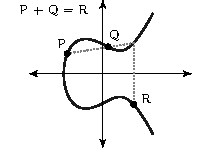
\includegraphics[scale=2]{tangent-and-chord}
		\caption{``tangent-and-add'' methode op een elliptische kromme\label{figuur-pairings-tangent-and-chord}}
\end{figure}

Aan de hand van de vorige bewerking kan een scalaire vermenigvuldiging vastgelegd worden, met $a \in \mathbb{Z}$:
\[\begin{aligned}
a \cdot A	&= A + \ldots + A\\
0 \cdot A	&= \mathcal{O}\\
-a \cdot A	&= a \cdot -A
\end{aligned}\]

De orde $n$ van een punt $A$ op de kromme is gelijk aan de minimum waarde waarvoor $n \cdot A = \mathcal{O}$. Het is mogelijk dat $n = \infty$. Van alle punten waarvoor $n$ een deler is van $l$ wordt gezegd dat ze in de $l$-torsiesubgroep van $E$ zitten. Zo een subgroep wordt genoteerd als:
\[E[l] = \{ A \in E : l \cdot A = \mathcal{O} \}.\]

Het aantal punten $\#E$ op $E$ wordt de orde van de kromme genoemd. Voor een kromme over een veld $\mathbb{F}_q$ is $\#E = q + 1 - t$, met $t$ de ``trace'' van de kromme. Indien $q \mid t$ wordt de kromme supersingulier genoemd. Voor bepaalde types krommen bestaat er een gesloten formule voor $\#E$.

Ten slotte wordt nog de Tate-inbeddingsgraad $k$ gedefinieerd. Stel $l \in \mathbb{Z}$ copriem aan $q$ zodat $E(\mathbb{F}_q)$ een punt van orde $l$ bevat. Dan is $k$ van $E$ tegenover $l$ gedefinieerd als het kleinste gehele getal waarvoor $l \mid q^k - 1$.

\section{Definitie van pairings}

Ten tijde van dit schrijven waren onder meer volgende pairings bekend: Weil, Tate, $\eta_T$ \cite{eta} en Ate \cite{ate}. In deze thesis zal gewerkt worden met de Tate pairing, waarvan bewezen is dat ze effici\"enter te berekenen is dan de Weil pairing.

De vermelde $\eta_T$ en Ate pairing zijn variaties op de Tate pairing die gebruikt kunnen worden indien voor specifieke elliptische krommen gekozen wordt. Indien aan de juiste voorwaarden voldaan wordt, zal de schakeling die in het volgende hoofdstuk wordt voorgesteld dus ook gebruikt kunnen worden om deze pairings te berekenen.

De Tate pairing is een functie $e(P, Q)$ met als argumenten twee punten uit een additieve groep en als resultaat een punt in een multiplicatieve groep:
\[e(P, Q): \mathbb{G}_1 \times \mathbb{G}_2 \mapsto \mathbb{G}_T.\]
Een pairing moet tevens volgende eigenschappen bezitten: goed gedefinieerd, non-degenererend en bilineariteit. Het is de combinatie van deze drie eigenschappen die het zo moeilijk maakt de pairing te defini\"eren. De betekenis van deze drie eigenschappen is:
\begin{enumerate}
	\item Goed gedefinieerd: $e(\mathcal{O}, Q) = 1 \: \forall \: Q \in \mathbb{G}_2$; $e(P, \mathcal{O}) = 1 \: \forall \: P \in \mathbb{G}_1$.
	
	\item Non-degenererend: $\forall \: P \in \mathbb{G}_1, \: \exists \: Q \in \mathbb{G}_2$ waarvoor $e(P, Q) \neq 1$.
	
	\item Bilineariteit: $\forall \: P_1, P_2, P \in \mathbb{G}_1$ en $\forall \: Q_1, Q_2, Q \in \mathbb{G}_2$ geldt:
		\[\begin{aligned}
			e(P_1 + P_2, Q) &\equiv e(P_1, Q) \cdot e(P_2, Q) \qquad \text{ en }\\
			e(P, Q_1 + Q_2) &\equiv e(P, Q_1) \cdot e(P, Q_2).
		\end{aligned}\]
\end{enumerate}

De Tate pairing over elliptische krommen wordt als volgt geschreven:
\[e(P, Q): E(\mathbb{F}_{q^k})[l] \times E(\mathbb{F}_{q^k})/l E(\mathbb{F}_{q^k}) \mapsto \mathbb{F}_{q^k}^* / (\mathbb{F}_{q^k}^*)^l.\]

Het resultaat van de Tate pairing is niet uniek, maar een element van een equivalentieklasse $\mathbb{F}_{q^k}^* / (\mathbb{F}_{q^k}^*)^l$. Voor twee resultaten $a, b \in \mathbb{F}_{q^k}^*$ geldt $a \equiv b$ als en slechts als er een element $c \in \mathbb{F}_{q^k}^*$ waarvoor $a = bc^l$. Aangezien voor cryptografische toepassingen een uniek resultaat gewenst zal zijn, dient die $n$-de macht weggewerkt te worden. Dit kan door het resultaat te verheffen tot de macht $\frac{q^k - 1 }{l}$. Aangezien $a^{q^k - 1} = 1$ voor elke $a \in \mathbb{F}_{q^k}^*$ (kleine stelling van Fermat), verkrijgt men dan dus een $l$-eenheidswortel. Soms wordt over de gereduceerde Tate pairing gesproken wanneer men expliciet wil aangeven dat deze machtsverheffing wordt uitgevoerd.

Het formeel bewijzen van de Tate pairing valt buiten het bestek van deze thesis. Voor meer informatie wordt onder andere verwezen naar \cite{maas, ruck, hess}.

\section{Berekening van de Tate pairing\label{sectie-pairings-berekening}}

Reeds in 1986 stelde Miller een methode voor om de Tate pairing te berekenen \cite{miller, barreto-efficient}. \refalg{algoritme-pairings-miller} geeft weer hoe dat algoritme werkt.

\begin{algorithm}[h]
	\caption{Millers algoritme voor de Tate pairing}
	\label{algoritme-pairings-miller}
	\KwIn{$l \in \mathbb{Z}$; $P, Q \in E(\mathbb{F}_{q^k})[l]$}
	\KwOut{$e(P, Q) \in \mathbb{F}_{q^k}^*$}
	\KwData{$i, t \in \mathbb{Z}$; $F, Q', S, V \in \mathbb{F}_{q^k}$}
	$t \gets \left\lfloor \log _2 (l) \right\rfloor$\;
	$Q' \gets \textsf{rand}(E)$\;
	$S \gets Q + Q'$\;
	$F \gets 1$; $V \gets P$\;	
	\For{$i = t - 1$ to $0$}{
		$F \gets F^2 \cdot \frac{G_{V,V}(S) \cdot G_{2 \cdot V}(Q')}{G_{2 \cdot V}(S) \cdot G_{V,V}(Q')}$\;
		$V \gets 2 \cdot V$\;
		\If{$l_i = 1$}{
			$F \gets F \cdot \frac{G_{V,P}(S) \cdot G_{V + P}(Q')}{G_{V + P}(S) \cdot G_{V,P}(Q')}$\;
			$V \gets V + P$\;
		}
	}
	\KwRet{$F^{\frac{q^k - 1 }{l}}$}
\end{algorithm}

Daarbij staat $G_{A, B}(C)$ voor de evaluatie van het punt $C$ in de vergelijking van de rechte door de punten $A$ en $B$. Indien $G_{2 \cdot A}$ vermeld staat, wil dit de vergelijking door de raaklijn aan $2 \cdot A$ zeggen.

Hoewel als argumenten van het algoritme elementen van $\mathbb{F}_{q^k}$ staan aangegeven, zal doorgaans voor elementen uit het subveld $\mathbb{F}_q$ gekozen worden. Het resultaat van de pairing zal dus $k$ keer groter zijn dan de opgegeven argumenten. 

In \cite{barreto-efficient} wordt aangetoont dat indien gewerkt wordt in het veld $\mathbb{F}_{2^m}$ het algoritme sterk vereenvoudigd kan worden. Er moet dan gebruik gemaakt worden van de supersinguliere kromme
\[E(\mathbb{F}_{2^m}): y^3 + y = x^3 + x + b\]
met $b \in \{0, 1\}$. Verder dient ook een distortiemap $\phi$ toegepast te worden op het punt $Q$. Voor een veld $\mathbb{F}_{2^m}$ dient de mapping te voldoen aan volgende voorwaarden:
\[\phi : (x_Q, y_Q) \mapsto (x_Q + s^2, y_Q + x_Q s + t^6)\]
met $s, t \in \mathbb{F}_{2^{km}}$. Daarbij moeten $s$ en $t$ voldoen aan volgende vergelijkingen:
\[\left\{\begin{array}{l}
s^4 + s = 0\\
t^2 + t + s^6 + s^2 = 0
\end{array}\right.\]

Een bijkomend voordeel van het gebruik van de vermelde kromme is haar lage inbeddingsgraad $k = 4$. Hoe groter $k$, hoe meer bewerkingen het immers kost om de pairing te berekenen. Tevens zorgt de distortiemap er voor dat $e(P, P) \neq 1$, wat wordt omgeschreven als sterk niet-degenererend.

De resulterende effici\"entere versie van Millers algoritme is gegeven in \refalg{algoritme-pairings-miller-beter}.
Het is de combinatie van deze drie eigenschappen die het zo moeilijk maakt de pairing te defini\"eren.
\begin{algorithm}[h]
	\caption{Millers algoritme voor de Tate pairing - Effici\"entere versie}
	\label{algoritme-pairings-miller-beter}
	\KwIn{$l \in \mathbb{Z}$; $P, Q \in E(\mathbb{F}_{2^m})[l]$}
	\KwOut{$e(P, Q) \in \mathbb{F}_{2^{km}}^*$}
	\KwData{$i, t \in \mathbb{Z}$; $F, V \in \mathbb{F}_{2^{km}}$}
	$t \gets \left\lfloor \log _2 (l) \right\rfloor$\;
	$F \gets 1$; $V \gets P$\;	
	\For{$i = t - 1$ to $0$}{
		$F \gets F^2 \cdot G_{V,V}(\phi(Q))$\;
		$V \gets 2 \cdot V$\;
		\If{$l_i = 1$ en $i \neq 0$}{
			$F \gets F \cdot G_{V,P}(\phi(Q))$\;
			$V \gets V + P$\;
		}
	}
	\KwRet{$F^{\frac{2^{km} - 1 }{l}}$}
\end{algorithm}

\section{Veiligheid van pairings}

Nu de wiskundige achtergrond van de Tate pairing enigszins verduidelijkt is, zal getoond worden waarom pairings veilig genoeg zijn om gebruikt te kunnen worden in cryptografische toepassingen.

Eerst dienen echter de begrippen een moeilijk en een gemakkelijk probleem gedefinieerd te worden. Een moeilijk probleem is een probleem waarvoor geen algoritme bekend is dat een oplossing kan vinden in polynomiale tijd. Voor een gemakkelijk probleem bestaan er wel algoritmen die in polynomiale tijd een oplossing leveren.

De veiligheid van pairings vindt zijn oorsprong in het discrete logaritme (DL) probleem. Dit wordt gedefinieerd als volgt. Definieer de multiplicatieve groep $\mathbb{G}$ van orde $n$, met $n$ priem en $g$ een generator voor $\mathbb{G}$. Stel nu $h \in \mathbb{G}$ en dat $n$ priem is. In theorie is het niet nodig dat $n$ priem is. Indien dit niet het geval is, kan het probleem echter gereduceerd worden tot een probleem met $n$ priem via de Chinese reststelling. Stel nu $x \in \mathbb{Z}_n^*$, zodat $h = g^x$. Het discrete logaritme probleem bestaat er dan in $x$ te vinden, gegeven $g$ en $h$. Dit wordt geschreven als DL$(h) = x$.

Het DL probleem wordt algemeen aanzien als moeilijk. De snelste algoritmes die dit probleem kunnen oplossen voor een willekeurige groep $\mathbb{G}$ (d.w.z.\ die geen specifieke eigenschappen van het veld uitbuiten) hebben een complexiteit $O(\sqrt{n})$, met $n$ de orde van de groep. Aangezien $n$ exponentieel groeit met de grootte van de groep, geldt hetzelfde voor de uitvoeringstijd van de algoritmes. Enkele voorbeelden van zulke algoritmes zijn Baby-step giant-step \cite{baby-step} en Pollards rho algoritme \cite{pollard-rho}. Voor bepaalde groepen zijn algoritmes bekend met subexponenti\"ele tijdscomplexiteit. In het geval de groep gedefinieerd is als de punten op een supersinguliere elliptische krommen, kan men bijvoorbeeld MOV- \cite{mov} of FR-reductie \cite{ruck} gebruiken. In dat geval is het noodzakelijk de grootte van de groep waarover de kromme gedefinieerd is groot genoeg te nemen, zodat het computationeel onhaalbaar blijft het DL probleem op te lossen.

Een probleem verwant aan het DL probleem is het computationele Diffie-Hellman (CDH) probleem. Stel $a, b \in \mathbb{Z}^*_n$. In dit geval worden $g, g^a, g^b \in \mathbb{G}$ gegeven. Het probleem is nu een element $h \in \mathbb{G}$ te vinden waarvoor $h = g^{ab}$. Het probleem wordt uitgedrukt als CDH$(g^a, g^b) = h$.

Aangezien het CDH probleem kan opgelost worden indien het DL probleem kan opgelost worden, is het dus zeker niet moeilijker. Indien het CDH probleem moeilijk is, is het DL probleem dat dus ook. Of het omgekeerde geldt, is niet geweten. Tot nu toe zijn echter geen methodes gekend die het CDH probleem sneller oplossen dan de methodes die het DL probleem oplossen. De twee worden dan ook als equivalent beschouwd.

Ten derde is er dan het beslissings Diffie-Hellman (DDH) probleem. Stel $a, b, c \in \mathbb{Z}^*_n$. Nu dient, gegeven $g, g^a, g^b, g^c \in \mathbb{G}$, beslist te worden of $g^c = g^{ab} \: (\bmod \: n)$. Dit wordt uitgedruk als DDH$(g^a, g^b, g^c) = 1$ indien waar en DDH$(g^a, g^b, g^c) = 0$ in het andere geval.

Het DDH probleem kan opgelost worden aan de hand van het CDH probleem door $h =$ CDH$(g^a, g^b)$ te berekenen en na te gaan of $h = g^c$. Het is dus duidelijk dat het DDH probleem zeker niet moeilijker is dan het CDH probleem. Er zijn echter bepaalde groepen bekend waarvan geweten is dat het DDH probleem makkelijk is en het CDH probleem moeilijk. Deze groepen worden ``gap Diffie-Hellman'' groepen genoemd. Pairings genereren zo een groep, het CDH probleem over elliptische krommen wordt immers als moeilijk beschouwd en ze laten toe DDH$(aP, bP, cP)$ makkelijk te beantwoorden:
\[\begin{aligned}
e(aP, bP) &= e(P, bP)^a\\
								&= e(P, abP)\\
								&= e(P, cP)
\end{aligned}\]
%\[e(aP, b P) &= e(P, b P)^a = e(P, ab  P) = e(P, c P)\]
als en slechts als $ab = c$.

\section{Toepassingen van pairings}

Hoewel de theorie van pairings enigszins is uitgelegd, blijft nog steeds de vraag hoe van hun eigenschappen gebruik gemaakt kan worden in cryptografische algoritmen. In deze paragraaf zullen enkele mogelijkheden voorgesteld worden. Opnieuw wordt er op gewezen dat dit zeker geen volledige lijst van mogelijkheden is en meer informatie te vinden is in \cite{maas}.

\subsection{Encryptie}

Verschillende encryptieschema's met pairings zijn bekend. Hier wordt BasicIdent voorgesteld, het eerste bekende schema voor identiteits-gebaseerde encryptie, in 2001 gepubliceerd door Boneh en Franklin \cite{boneh}. Het schema bestaat uit vier algoritmen. Het eerste, `setup', initialiseert de systeemparameters, waaronder de geheime hoofdsleutel voor de centrale server. Ten tweede is er het `extract' algoritme dat gebruikt wordt om gebruikers te voorzien van een geheime sleutel. De laatste twee, `encrypt' en `decrypt', laten toe, zoals de naam het zegt, berichten te versleutelen en ontcijferen. De vier algoritmen worden hieronder verder uitgelegd.

\paragraph{Setup} Eerst wordt een $k$-bit lang priemgetal $q$ gekozen. Er wordt een additieve en een multiplicatieve groep van orde $q$ gedefinieerd, respectievelijk $\mathbb{G}_1$ en  $\mathbb{G}_2$. Ten slotte is er nog een generator $P$ van $\mathbb{G}_1$ nodig.

Vervolgens wordt de geheime hoofdsleutel $s \in \mathbb{Z}^*_q$ van de server willekeurig gekozen en stelt men $P_{\text{pub}} = sP$. Tevens is er nood aan twee cryptografische hashfuncties: $H_1 : \{ 0,1 \}^* \mapsto \mathbb{G}_1^*$ en $H_2 : \mathbb{G}_2 \mapsto \{ 0, 1 \}^n$. De waarde van $n$ kan willekeurig gekozen worden en zal de lengte van het te versleutelen bericht bepalen. Deze waarde heeft dus geen invloed op de veiligheid van het systeem.

Een bericht $M = \{ 0,1 \}^n$ en de sleuteltekst $C \in \mathbb{G}_1^* \times \{ 0,1 \}^n$.

De publieke systeemparameters zijn: $q$, $\mathbb{G}_1$, $\mathbb{G}_2$, $n$, $P$, $P_{\text{pub}}$, $H_1$ en $H_2$. Elke gebruiker heeft toegang tot deze parameters.

\paragraph{Extract} De server berekent een gebruiker zijn geheime sleutel als:
\[d_{\text{ID}} = s Q_{\text{ID}},\]
met $Q_{\text{ID}} = H_1(\text{ID})$. ID is een bitstring die uniek de identiteit van de gebruiker bepaalt en $s$ de geheime hoofdsleutel. Enkel de server kan dus geheime sleutels berekenen.

\paragraph{Encrypt} Kies een willekeurige $r \in \mathbb{Z}_q^*$ en stel $Q_{\text{ID}} = H_1(\text{ID})$. De sleuteltekst $C$ van bericht $M$ is dan:
\[C = \langle rP, M \xor H_2(g_{\text{ID}}^r) \rangle,\]
met $g_{\text{ID}}^r = e(Q_{\text{ID}}, P_{\text{pub}})$.

\paragraph{Decrypt} Een sleuteltekst $C = \langle U, V \rangle$ wordt ontcijfert als volgt:
\[M = V \xor H_2\big( e(d_{\text{ID}}, U) \big).\]
Dat het resultaat wel degelijk klopt is als volgt te bewijzen:
\[\begin{aligned}
e(d_{\text{ID}}, U)	&= e(sQ_{\text{ID}}, rP)\\
							&= e(Q_{\text{ID}}, P)^{sr}\\
							&= e(Q_{\text{ID}}, P_{\text{pub}})^r\\
							&= g_{\text{ID}}^r.
\end{aligned}\]
Het bericht $M$ ondergaat dus twee maal een exclusieve OR met $g_{\text{ID}}^r$.

Het is mogelijk uitbreidingen aan dit systeem toe te voegen. Zo kan bijvoorbeeld bij de berekening van iemands publieke sleutel een datum bij de ID gevoegd worden. De ontvanger dient de centrale server dan om een specifieke sleutel te vragen om het ontvangen berichten te ontcijferen. Afhankelijk van de datum van aanvraag kan de server deze aanvraag dan inwilligen of weigeren. Merk op dat in dit geval de ontvanger wel steeds de server moet contacteren alvorens ontcijfering mogelijk is.

%Buiten dit BasicIdent schema bestaat er ook een FullIdent schema dat extra veiligheid biedt in het geval een aanvaller de ontcijfering van enkele sleutelteksten kan bemachtigen. Dit wordt onder meer in detail besproken in \cite{maas}.

\subsection{Digitale handtekeningen}

Net zoals er verschillende schema's bestaan voor identeits-gebaseerde  encryptie, bestaan er ook verscheidene voor digitale handtekeningen. Hier wordt dat van Cha en Cheon \cite{cha} gepresenteerd. Opnieuw bestaat het schema uit vier algoritmes, `setup', `extract', `sign' en `verify'. Daarbij zijn de `setup' en `extract' algoritmes identiek aan die van het BasicIdent schema, met als extra publieke parameter een hashfunctie $H_3 : \{ 0,1 \} ^* \times \mathbb{G}_1 \mapsto \mathbb{Z}_q ^*$. De `sign' en `verify' algoritmes werken als volgt:

\paragraph{Sign} Kies een willekeurige $r \in \mathbb{Z}_q^*$ en bereken $U = r Q_{\text{ID}}$. Stel vervolgens $h = H_3(M, U)$ en $V = (r + h) \cdot d_{\text{ID}}$. De handtekening is dan $\sigma = \langle U, V \rangle$.

\paragraph{Verify} Een handtekening bij een bericht $M$ is geldig indien
\[e(P, V) = e(P_{\text{pub}}, U + h Q_{\text{ID}}),\]
met $h$ zoals gedefinieerd in het `sign' algoritme. Dat dit klopt kan geverifieerd worden als volgt:
\[\begin{aligned}
e(P, V)	&= e(P, (r + h) \cdot d_{\text{ID}})\\
			&= e(P, (r + h) \cdot s Q_{\text{ID}})\\
			&= e(P, (r + h) \cdot Q_{\text{ID}})^s\\
			&= e(P_{\text{pub}}, U + h Q_{\text{ID}})\\
\end{aligned}\]

\subsection{Sleutelafspraak}

Naast sleutelafspraak zoals die bestaat in publieke sleutelcryptografie laten pairings enkele opmerkelijke schema's toe om sleutels af te spreken. Twee daarvan worden hier gepresenteerd.

\subsubsection{Niet-interactieve sleutelafspraak}

Een niet-interactief sleutelafspraak is een sleutelafspraak waarbij de betrokken partijen geen contact met elkaar dienen op te nemen om de sleutel af te spreken. Dit heeft als voordeel dat een man-in-the-middle aanval onmogelijk is. Volgende techniek werd voorgesteld in \cite{sakai}. Twee partijen A en B spreken een gezamenlijke sleutel $k$ af door middel van volgende formules:
\[\begin{aligned}
k	&= e(d_{\text{A}}, Q_{\text{B}})\\
	&= e(s Q_{\text{A}}, Q_{\text{B}})\\
	&= e(Q_{\text{A}}, d_{\text{B}}).\\
\end{aligned}\]

Aangezien beiden hun persoonlijke geheime sleutel bezitten en de publieke sleutel van de andere persoon kunnen berekenen, is er dus geen communicatie noodzakelijk. Een nadeel van dit schema is dat de afgesproken sleutel steeds dezelfde zal zijn. In \cite{smart} wordt een schema voorgesteld om de sleutel dynamisch te maken, daarbij is echter wel communicatie vereist.

\subsubsection{Driepartijdige sleutelafspraak}

Met behulp van pairings is het mogelijk tussen drie partijen een sleutel af te spreken in slechts \'e\'en communicatieronde \cite{joux}, daar waar er normaal minstens twee rondes nodig zijn. Dit gaat als volgt in zijn werk: de drie partijen publiceren respectievelijk $aP$, $bP$ en $cP$, met willekeurige $a, b, c \in \mathbb{Z}_q^*$. De gedeelde geheime sleutel $k$ is dan:
\[\begin{aligned}
k	&= e(bP, cP)^a\\
	&= e(aP, cP)^b\\
	&= e(aP, bP)^c\\
	&= e(P, P)^{abc}
\end{aligned}\]
Merk op dat dit schema geen gebruik maakt van identiteiten en dus niet tot identiteits-gebaseerde cryptografie behoord. Tevens is het niet bestand tegen man-in-the-middle aanvallen. In \cite{paterson} wordt met behulp van publieke sleutel cryptografie een resistent schema uitgewerkt.
